\documentclass{article}
\PassOptionsToPackage{numbers,sort&compress}{natbib}
\usepackage[preprint]{neurips_2026}
\usepackage[T1]{fontenc}
\usepackage{amsmath,amssymb,booktabs,longtable,tabularx,graphicx,xcolor}
\usepackage{microtype,float,listings}
\usepackage[colorlinks=true,linkcolor=blue!50!black,citecolor=blue!50!black,urlcolor=blue!50!black]{hyperref}
\setlength{\emergencystretch}{2em}
\lstset{basicstyle=\ttfamily\footnotesize,breaklines=true,breakatwhitespace=true,columns=fullflexible,
  keepspaces=true,showstringspaces=false,frame=single,rulecolor=\color{black!20},
  backgroundcolor=\color{black!2},aboveskip=0.6em,belowskip=0.6em}
\makeatletter
\newcommand{\tablerows}[1]{\@@input #1 }
\makeatother

\title{JEV-Star: Fast, Low-Cost StarCraft II Control\\with Language-Model Planning}
\author{%
  Weiyu Ma \quad Liangbing Zhao \quad Yongcheng Zeng$^{1}$ \quad Jian Zhao$^{2}$\\
  $^{1}$Institute of Automation, Chinese Academy of Sciences\\
  $^{2}$Beijing Zhongguancun Academy\\
  \texttt{sc2meisah@gmail.com} \quad \texttt{jianzhao@zgci.ac.cn}
}

\begin{document}
\maketitle

\begin{abstract}
We present JEV-Star, a StarCraft II controller that defeats the strongest non-cheating built-in AI, Lv7, by combining fast JEV action selection with persistent GPT-6 planning. The combined system wins four full games at Lv5--Lv7, including two Lv7 victories with different seeds, while retaining a median JEV response time of 0.422 seconds. Mean estimated model cost across these games is USD~3.71 per game: USD~0.15 for JEV and USD~3.56 for GPT-6. We compare this system with an initial JEV-only controller in full-game macro control and multi-unit micromanagement. The standalone controller reaches a 20-minute limit against Lv2 without expanding. Across 35 battle maps with three episodes per map, the combined system raises mean enemy elimination from 16.50\% to 37.69\% and wins from 3 to 7 out of 105. Replay frames and decision logs connect these gains to resource reservation, persistent economic goals, and stable army objectives. The results demonstrate a practical division between inexpensive, subsecond decisions and longer-horizon planning. The comparison evaluates complete systems; concurrent interface improvements mean that planning's contribution is not isolated by a controlled ablation.
\end{abstract}

\section{Introduction}

StarCraft II requires both immediate decisions and commitments whose benefits arrive much later. A controller can repeatedly choose legal, affordable actions yet never save enough to expand its economy. It can also alternate between attacking and retreating without carrying either decision through. These failures motivate a separation between choosing the next action and maintaining a strategy.

We implement this separation with JEV, a hosted model that selects among structured alternatives \citep{typesafe2026jev}, and GPT-6, which supplies persistent strategic guidance. JEV remains responsible for frequent action selection. GPT-6 specifies goals, spending priorities, and conditions for changing army posture. The intended benefit is to preserve fast, low-cost interaction while using general-purpose planning where a single-step decision is insufficient.

JEV-Star builds on LLM Play SC2 for full-game control and SMAC-Hard for micromanagement \citep{ma2023textsc2,deng2024smachard}. We compare JEV-only with JEV + GPT-6. The combined controller achieves two victories against Lv7, the highest non-cheating difficulty of StarCraft II's built-in AI \citep{blizzard2026sc2protocol}. Our experiments measure game outcomes, response latency, and the combined model cost of a complete game. Replay frames and decision logs show how persistent plans change economic development and army behavior while preserving a fast action loop.

\section{Related work}

StarCraft II AI spans the SC2LE interface, full-game agents such as TStarBots, AlphaStar, TStarBot-X, and StarCraft Commander, and offline learning with AlphaStar Unplugged \citep{vinyals2017sc2le,sun2018tstarbots,vinyals2019alphastar,han2020tstarbotx,wang2020scc,mathieu2023unplugged}. Cooperative combat is studied in SMAC and its extensions, with methods including QMIX and MAPPO \citep{samvelyan2019smac,ellis2022smacv2,deng2024smachard,rashid2018qmix,yu2021mappo}. Our contribution concerns inference-time use of hosted models, without task-specific weight training.

LLM Play SC2 and LLM-PySC2 establish language-model interfaces for game control \citep{ma2023textsc2,li2024llmpysc2}. ReAct, Reflexion, Voyager, and SayCan connect reasoning or persistent context to executable actions \citep{yao2022react,shinn2023reflexion,wang2023voyager,ahn2022saycan}. AgentBench and WebArena emphasize evaluating interactive outcomes \citep{liu2023agentbench,zhou2023webarena}. JEV-Star uses a native choice interface for concrete actions and retains an explicit plan across decisions.

FrugalGPT and RouteLLM reduce cost through model selection, while ReWOO and LLMCompiler organize reasoning and tool execution \citep{chen2023frugalgpt,ong2024routellm,xu2023rewoo,kim2023llmcompiler}. We assign models by control role: frequent JEV actions and occasional GPT-6 plans. Our experiments examine this assignment through game performance, response latency, and per-game expenditure.

\section{Method}

\subsection{Structured action selection with JEV}

At decision time \(t\), the adapter constructs a structured observation \(x_t\) and an executable candidate set \(\mathcal{A}_t\). JEV selects an identifier:
\begin{equation}
    a_t = \operatorname{JEV}(x_t,\mathcal{A}_t).
\end{equation}
The executor validates the identifier, attempts the associated command, and includes recent outcomes in subsequent observations. Both methods use this loop; their difference is whether an explicit plan accompanies it (Figure~\ref{fig:architecture}).

For macro control, the observation summarizes resources, workers, buildings, technology, army composition, visible enemies, and recent actions. Candidates represent high-level commands such as producing a unit, constructing a building, researching an upgrade, expanding, attacking, retreating, or waiting. Local game code handles placement and low-level order execution. Feasibility checks consider prerequisites, supply, resources, and available producers. JEV chooses one command per request.

For micromanagement, the observation describes the team and visible enemies, including health, positions, ranges, cooldowns, and energy. Each living unit receives its own legal alternatives: move to an enumerated destination, attack an available target, heal an ally where supported, or stop. Unit choices share the same team observation and are submitted in concurrent batches. Execution returns information about rejected actions. This is centralized shared-vision control; it does not implement independently observed, decentralized MARL policies.

The JEV-only method selects directly from current state and short execution history. It has no separate process that maintains a future resource budget or a persistent team objective. In particular, an affordability filter can hide an expansion until sufficient minerals are available, even though reaching that threshold requires declining currently affordable purchases.

\begin{figure}[t]
\centering
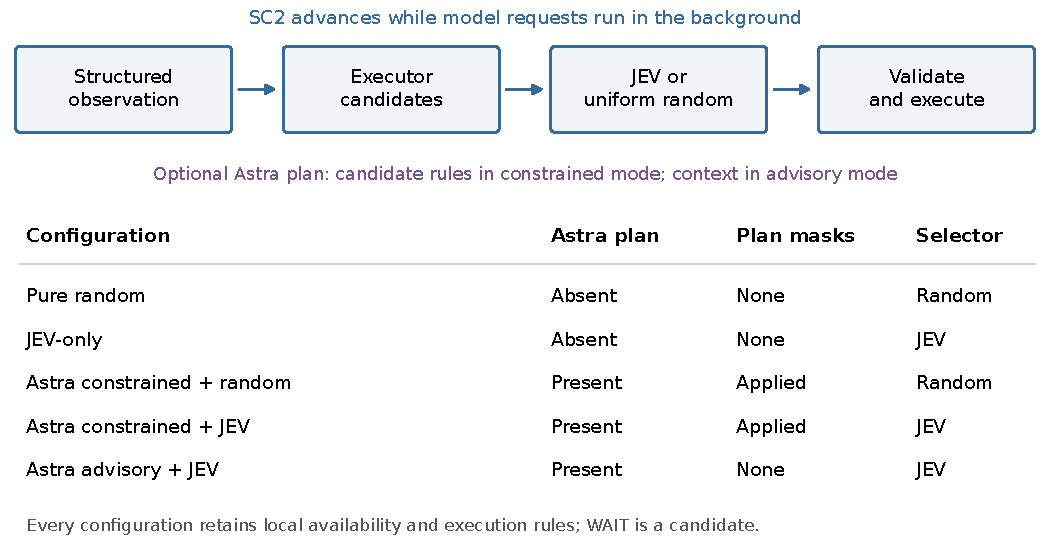
\includegraphics[width=\linewidth]{figures/architecture.pdf}
\caption{Two controllers with the same action loop. (a) JEV-only chooses executable actions from the current observation and recent feedback. (b) JEV + GPT-6 adds a plan that persists across action decisions. The plan supplies context to JEV and constrains macro candidates through resource reservations and army-posture rules. Micro plans provide tactical context while retaining legal unit choices. Macro and micro use separate game adapters.}
\label{fig:architecture}
\end{figure}

\subsection{Persistent planning with GPT-6}

In the combined method, a planner reads a state summary and, when available, the previous plan. It returns structured guidance \(z_k\), which remains active across multiple action decisions:
\begin{equation}
    z_k=\operatorname{GPT\text{-}6}(x_{t_k},z_{k-1}), \qquad
    a_t=\operatorname{JEV}(x_t,z_k,\widetilde{\mathcal{A}}_t), \quad
    t_k\leq t<t_{k+1}.
\end{equation}
The planner proposes goals rather than individual engine commands. Its output is checked before becoming active. A failed or delayed planning request leaves the previous valid plan available.

A macro plan specifies an economic objective, worker and base targets, production priorities, resource reservations, and an army posture. Resource reservation connects a future purchase to present action availability: when saving for an expansion, the adapter can suppress lower-priority spending until the required minerals accumulate. Emergency supply or defense actions can override these restrictions. Army guidance includes separate thresholds for starting and ending an attack and a minimum commitment interval, reducing repeated reversals near a single threshold. The plan enters both JEV's context and the adapter's candidate rules; the latter makes strategic commitments operational.

A micro plan describes conditional tactics and roles, such as which units should absorb pressure, which targets deserve priority, and when ranged units should reposition. One plan is generated for each map and reused for its three episodes. The legal action set remains available to JEV. A common plan provides shared intent, but independently chosen unit actions still lack a joint reservation mechanism for damage or healing targets.

\subsection{Control timing}

Full-game control is asynchronous: the game continues while requests are in flight. JEV requests are rate-limited to at most one per wall-clock second. The planner is checked on a nominal 60-game-second interval and at relevant events, subject to a minimum execution window. Completed plans are applied to subsequent decisions.

Micromanagement uses fixed-step interaction. The environment advances eight game loops only after a complete team decision has returned. Concurrent batching reduces waiting compared with sequential unit requests, but the slowest required response determines the next step. Consequently, model response latency and whole-episode wall time measure different parts of this system.

Neither method fine-tunes JEV or GPT-6. Both rely on the same division of responsibilities: game code determines observations and executable commands, JEV chooses actions, and the combined method adds GPT-6's persistent goals.

\section{Experiments}

\subsection{Setup and measurements}

We compare the initial JEV-only controller with the completed JEV + GPT-6 system. The runs use JEV 1.13, GPT-6 Astra with medium reasoning effort, and StarCraft II 5.0.16. Full-game experiments play Protoss against the built-in Zerg opponent on AltitudeLE, with eight starting workers. We report difficulty as Lv2, Lv5, Lv6, Lv7, or Lv8, following the ordered levels used by LLM Play SC2 \citep{ma2023textsc2}. The main sample contains one JEV-only game and four combined-system games; a completed Lv8 stress test is reported separately.

Micromanagement covers 35 local SMAC-Hard maps, with three episodes per map and method: 105 episodes each. Both methods use the same map configurations, game version, opponent controls, shared-vision setting, and disabled optional special abilities. Two local development maps are also excluded in a separate 33-map summary. There is one shared plan per map, so the three combined-method episodes do not represent independent planner samples. Candidate descriptions and execution handling also improved between the two controllers; these experiments measure the implemented systems rather than an isolated planner ablation.

We report wins, draws, losses, and mean enemy elimination, defined per episode as the fraction of initial enemy units eliminated. Each episode receives equal weight. For efficiency, we measure recorded response latency, total wall time, and model cost per complete episode. Macro outcomes and game durations are checked against replays. Cost estimates include recorded calls with known token usage, whether or not a returned plan was accepted.

\subsection{Full-game performance: defeating the strongest non-cheating AI}

Table~\ref{tab:macro} shows that JEV + GPT-6 wins all four completed ordinary-difficulty matches, including two victories against Lv7, the strongest built-in opponent without cheating advantages. These wins take 10:49--15:55 of game time. The first attacks occur between 7:22 and 8:11, following an economic and production buildup. JEV-only reaches its 20-minute game-time limit without a win. The two Lv7 seeds establish successful play at the highest non-cheating difficulty, although the sample is too small to estimate a reliable win rate.

\begin{table}[t]
\caption{Completed full-game experiments (times in minutes:seconds). The first five rows form the main comparison. The final Lv8 row is a separate stress test against an opponent with an information advantage. A time limit is not a victory.}
\label{tab:macro}
\centering\small
\begin{tabular}{llclrr}
\toprule
Method & Difficulty & Seed & Outcome & Game time & Wall time \\
\midrule
\tablerows{tables/study_macro_results.tex}
\bottomrule
\end{tabular}
\end{table}

Figure~\ref{fig:lv7replay} shows four moments from the Lv7 seed-1 victory: expansion, army movement, pressure on a Zerg base, and the final push. The frames come from the evaluated replay, rendered afterward with an observer camera. This viewing perspective supplies illustrations only; the controller acts on structured observations, not these images.

\begin{figure}[tp]
\centering
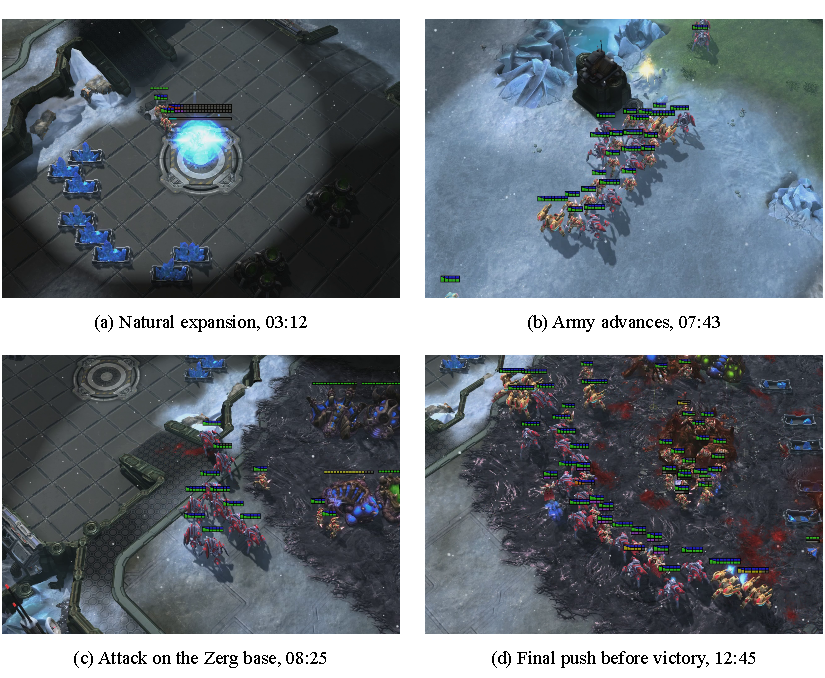
\includegraphics[width=\linewidth]{figures/lv7_replay.pdf}
\caption{Actual replay frames from JEV + GPT-6 defeating Lv7 on AltitudeLE, seed 1. (a) The natural Nexus is under construction. (b) The army advances after the logged attack command at 07:33. (c) Units attack the Zerg base. (d) The push continues shortly before victory at 12:48. Displayed times are game time, rounded to the nearest second. The replay observer view is used only for presentation.}
\label{fig:lv7replay}
\end{figure}

LLM Play SC2 reports its main evaluation at Lv5 (12 wins in 20 games for GPT-4-Turbo); a separate GPT-3.5 prompt study reaches Lv6 with an 8.33\% win rate \citep{ma2023textsc2}. Our Lv7 victories exceed the demonstrated difficulty in those reported experiments. The game versions and starting conditions differ, so this is a difficulty milestone rather than a matched win-rate comparison. That paper does not provide directly comparable per-game model charges or response latencies; we therefore quantify JEV-Star's speed and expenditure from our own logs in Section~\ref{sec:efficiency}.

\paragraph{Stress test with privileged vision.}
We additionally test Lv8, whose built-in opponent has a vision advantage. This game ends in defeat at 10:14. At five minutes, the agent's army resource value is 900 versus the opponent's 1,525; its first Immortal appears only at 6:25. It never issues an attack command. This failure illustrates a remaining economic--military imbalance when facing a stronger, privileged opponent; it is separate from the non-cheating difficulty milestone.

\subsection{Micromanagement: better damage, limited conversion to wins}

Table~\ref{tab:micro} summarizes the complete 35-map comparison. Mean enemy elimination rises from 16.50\% to 37.69\%, an increase of 21.19 percentage points, or 2.28 times the initial value. Wins increase from 3 to 7 out of 105. Excluding the two development maps retains the same win counts and increases mean elimination from 15.55\% to 39.17\%. The improvement is therefore not driven by those maps.

\begin{table}[t]
\caption{Micromanagement outcomes. Elimination is the episode-average fraction of enemy units eliminated. The 33-map subset excludes two local development maps. Both methods use three episodes per map.}
\label{tab:micro}
\centering\small
\begin{tabular}{lrrrr}
\toprule
& \multicolumn{2}{c}{All 35 maps: 105 episodes} & \multicolumn{2}{c}{33 maps: 99 episodes} \\
\cmidrule(lr){2-3}\cmidrule(lr){4-5}
Method & W/D/L & Elimination & Wins & Elimination \\
\midrule
\tablerows{tables/study_micro_results.tex}
\bottomrule
\end{tabular}
\end{table}

The combined system improves mean elimination on 25 maps, ties on seven, and declines on three (Figure~\ref{fig:micro}). On \texttt{mmmt}, elimination increases from 3.03\% to 87.88\% and wins from zero to two. On \texttt{MMM}, it rises from 10.00\% to 73.33\%, with one win; \texttt{8m} and \texttt{2c\_vs\_64zg} also acquire wins. These cases indicate a useful change in tactical behavior beyond merely issuing valid actions.

Nevertheless, the combined system still loses 98 episodes. On \texttt{3m}, elimination increases from zero to 66.67\% without a win. On \texttt{2s3z}, wins decline from two to one; on \texttt{bane\_vs\_bane}, elimination declines from 100\% to 77.78\%. Planning helps many battles but does not consistently convert local damage into team survival and victory.

Appendix~\ref{app:replays} presents paired frames from the first \texttt{mmmt} episode of each method, together with the combined controller's tactical guidance and recorded outcome. These examples illustrate the quantitative results; they are not additional evaluation episodes.

\begin{figure}[t]
\centering
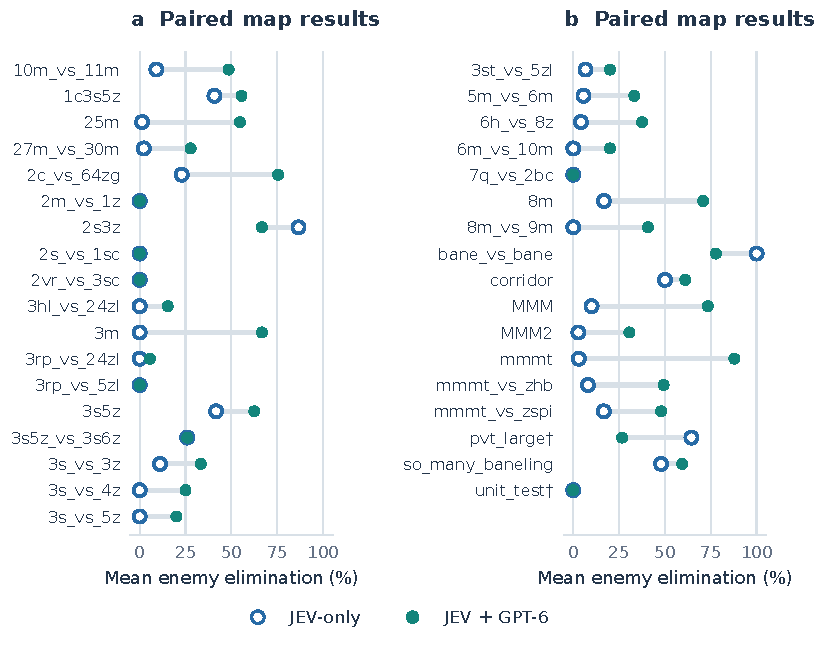
\includegraphics[width=\linewidth]{figures/micro_comparison.pdf}
\caption{Mean enemy elimination on all 35 maps, with three episodes per point. A connecting line pairs the two methods on the same map. The combined system improves 25 maps, ties seven, and declines on three. Daggers mark the two local development maps excluded from the 33-map summary.}
\label{fig:micro}
\end{figure}

\subsection{Why does planning help?}
\label{sec:behavior}

\paragraph{Saving for a future goal.}
The initial JEV-only full game illustrates a failure of longer-horizon resource allocation. It grows to 68 workers but remains on one base for the entire 20 minutes. Across 1,024 requests, the largest observed mineral balance is 335, below the 400 required for a Nexus. Expansion is consequently absent from every candidate set. Repeated affordable purchases prevent the saving needed to make the strategic action available.

The first accepted plan in a combined-system game requests two bases and instructs the controller to stop worker growth near 19 workers while saving for the natural expansion. The adapter turns this instruction into a spending reservation. Across the four wins, a second Nexus is first observed at 2:50--3:05, and peak observed base counts reach four to six. Figure~\ref{fig:planning} contrasts the economic and army trajectories. The useful contribution of planning is an explicit future target plus a mechanism that protects the resources needed to reach it.

This evidence diagnoses the initial controller's planning limitation, rather than showing that JEV can never reason about expansion. The affordability filter and one-step objective interact: neither exposes the value of temporarily refusing purchases. The combined system supplies that missing context and commitment.

Table~\ref{tab:replaytrace} follows the same Lv7 game shown in Figure~\ref{fig:lv7replay}. The log connects a request to prioritize the natural expansion, JEV's choice when 400 minerals become available, and the subsequent appearance of a second Nexus. An attack plan later produces 24 unit orders within one game second. This trace distinguishes model intent, command submission, and observed game state. Selected original fields appear in Appendix~\ref{app:replays}.

\begin{table}[t]
\caption{Plan--decision--execution trace from the Lv7 seed-1 victory. Rows summarize contemporaneous logs; time is minutes:seconds.milliseconds. A submitted building order is followed by an independent observation of construction.}
\label{tab:replaytrace}
\centering\small
\setlength{\tabcolsep}{4pt}
\begin{tabularx}{\linewidth}{llX}
\toprule
Game time & Source & Recorded behavior \\
\midrule
\tablerows{tables/replay_macro_trace.tex}
\bottomrule
\end{tabularx}
\end{table}

\paragraph{Maintaining an army objective.}
In the same JEV-only game, six attack commands and seven retreat commands include five attack-to-retreat reversals within two game seconds. Such rapid reversals leave little time for an attack to make progress. None of the four combined-system wins contains a reversal within that interval. Persistent posture, separate attack and retreat thresholds, and a commitment window stabilize the objective across JEV calls. Peak observed army supply rises from 58 in the standalone run to 79--129 in the combined games. Different opponents and other controller changes preclude a causal estimate, but the traces are consistent with better strategic continuity.

\begin{figure}[t]
\centering
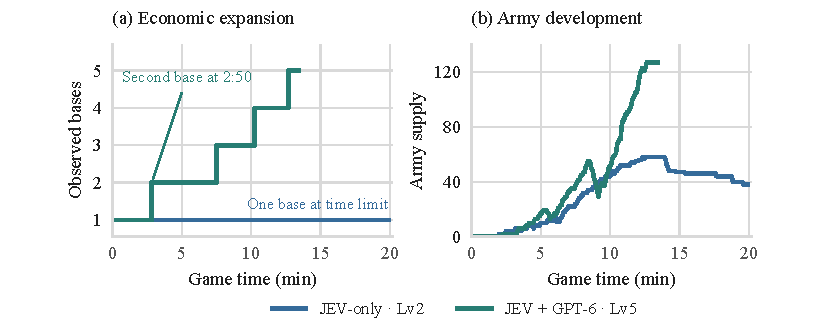
\includegraphics[width=\linewidth]{figures/planning_behavior.pdf}
\caption{Example full-game trajectories: JEV-only at Lv2 and JEV + GPT-6 at Lv5. The standalone controller remains on one base; the combined controller saves for expansion and develops a larger army. Base counts include structures under construction, and army supply can include pending production. The different opponents make this a behavioral illustration, not a controlled ablation.}
\label{fig:planning}
\end{figure}

\paragraph{Shared intent does not resolve all coordination.}
Micromanagement reveals a different boundary. In the combined system, 2,629 of 2,662 unit decisions with a ready weapon and an available in-range target choose an in-range attack. Basic engagement is usually sensible. However, among 930 decisions with a long weapon cooldown, nearby melee pressure, and an available movement endpoint that increases separation, 794 continue attacking and only 63 choose such a separating endpoint. The controller often fails to use movement during downtime.

Healing exposes resource conflicts between units. Execution records contain 500 healing rejections because a target is already targeted and ten for insufficient energy. Among 378 subsequent decisions that expose a previously rejected healing target together with an alternative legal target, 243 repeat the previous target. These conditional counts identify recurring behavior, not optimal-action labels. They suggest that planning alone cannot replace precise cooldown control, updated execution feedback, or joint allocation of healing targets.

\subsection{Response time and cost per game}
\label{sec:efficiency}

\paragraph{Frequent actions remain subsecond.}
Table~\ref{tab:latency} and Figure~\ref{fig:latency} report response distributions. Median JEV latency is 0.406 seconds for standalone macro control and 0.422 seconds with planning; corresponding micro medians are 0.485 and 0.500 seconds. In the combined system, macro and micro JEV 95th percentiles are 0.531 and 0.594 seconds. GPT-6 planning is less frequent but slower: median latency is 27.60 seconds in macro control and 37.17 seconds in micromanagement. These are different computational roles and inputs, so their ratio is not a same-task model speedup. The practical benefit is that most actions proceed through the faster decision layer.

\begin{table}[t]
\caption{Pooled latency over recorded responses with known usage. Macro JEV + GPT-6 statistics cover the four ordinary-difficulty wins; the Lv8 stress test is excluded. Micro statistics cover 105 episodes per method and 35 shared plans for the combined method.}
\label{tab:latency}
\centering\small
\begin{tabular}{llrrrr}
\toprule
& & \multicolumn{2}{c}{JEV action responses} & \multicolumn{2}{c}{GPT-6 planning responses} \\
\cmidrule(lr){3-4}\cmidrule(lr){5-6}
Setting & Method & \(n\) & P50/P95 (s) & \(n\) & P50/P95 (s) \\
\midrule
\tablerows{tables/study_latency.tex}
\bottomrule
\end{tabular}
\end{table}

\begin{figure}[t]
\centering
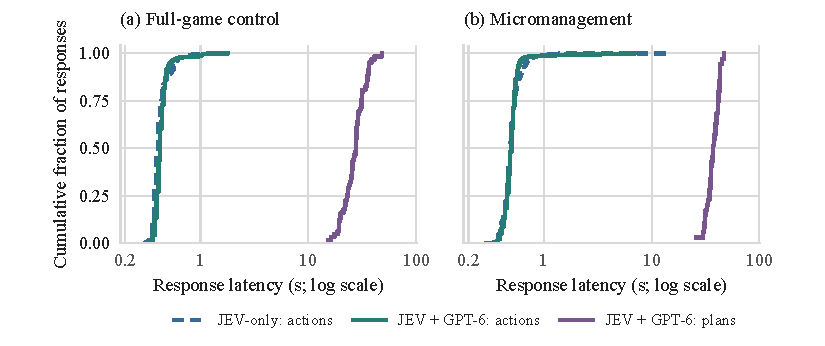
\includegraphics[width=\linewidth]{figures/response_latency.pdf}
\caption{Response-latency distributions by role and method. Both methods retain subsecond median JEV responses. GPT-6 provides less frequent, more expensive planning calls. The horizontal axis is logarithmic; each curve pools responses within its setting.}
\label{fig:latency}
\end{figure}

\paragraph{A complete game includes both models.}
Figure~\ref{fig:costs} shows the cost of each full game and the average micro episode, separating JEV, GPT-6, and their total. Across the four full-game wins, combined cost ranges from USD~2.83 to USD~4.52 and averages USD~3.7103. JEV accounts for USD~0.1499 per game and GPT-6 for USD~3.5604: planning contributes 96.0\% of the total. JEV's recorded macro usage costs approximately USD~0.21 per 1,000 responses. Cheap action selection therefore supports frequent interaction, while the planning schedule determines most of the game's model expenditure.

\begin{table}[t]
\caption{Mean model cost and elapsed wall time per completed episode. Macro averages use the main full-game sample. Micro planner cost and setup time are amortized over three episodes per map. Costs are known-usage standard-API-equivalent estimates, not billing statements.}
\label{tab:costs}
\centering\small
\setlength{\tabcolsep}{4pt}
\begin{tabular}{llrrrrr}
\toprule
& & & \multicolumn{3}{c}{USD per episode} & Wall time \\
\cmidrule(lr){4-6}
Setting & Method & Episodes & JEV & GPT-6 & Total & (s/episode) \\
\midrule
\tablerows{tables/study_costs.tex}
\bottomrule
\end{tabular}
\end{table}

\begin{figure}[t]
\centering
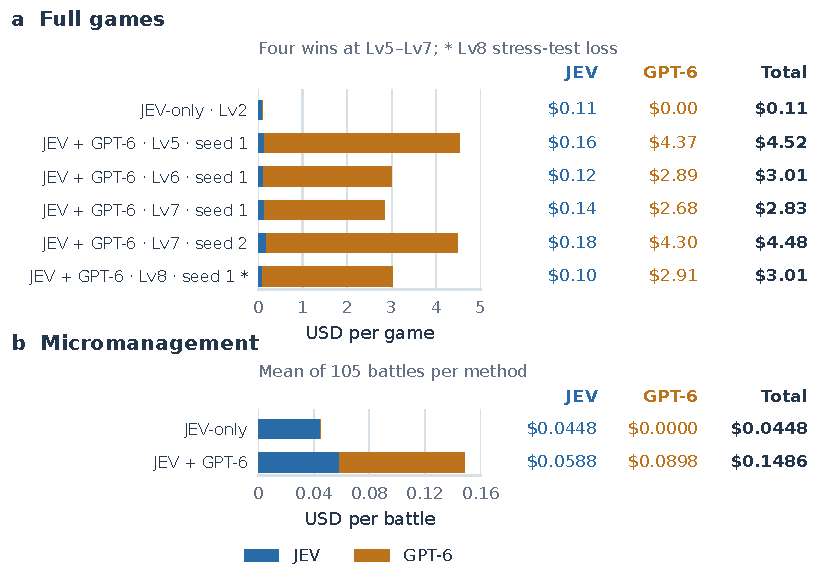
\includegraphics[width=\linewidth]{figures/game_costs.pdf}
\caption{Cost per game, with model components and totals. Top: each completed full-game experiment, including the separate Lv8 defeat. Bottom: mean battle cost over 105 episodes per method, amortizing each map's planning call across three episodes. Components and totals are rounded independently. Missing usage remains unpriced.}
\label{fig:costs}
\end{figure}

For micromanagement, standalone JEV costs USD~0.0448 per episode. The combined method costs USD~0.1486, consisting of USD~0.0588 for JEV and USD~0.0898 for planning. Excluding the two development maps gives USD~0.0243 and USD~0.1168, respectively. The combined method thus spends more than JEV-only while producing better aggregate combat outcomes. Its advantage is improved capability with an inexpensive action layer, not a reduction in the total charge relative to the standalone controller.

Mean micro wall time increases from 25.78 to 46.23 seconds per episode. This includes amortized planning, environment setup, stepping, and cleanup. Macro games run in real time while inference overlaps game execution, and their durations also depend on when a match ends. Neither shorter successful games nor the difference between action and planning latency alone establishes a full-game speedup over prior systems.

\paragraph{Accounting basis.}
We price recorded token usage at the providers' standard rates on September 22, 2026 \citep{typesafe2026models,openai2026gpt6astra}. JEV charges for input; GPT-6 accounting separates cached from uncached input and includes output tokens. Reasoning output is a subset of output, not an additional charge. GPT-6 runs use Codex, so the reported amount is an equivalent API estimate. Calls without usage remain unpriced; Appendix~\ref{app:costs} gives token totals, missing-call counts, and per-game figures.

\section{Discussion and limitations}

The experiments support a specific explanation for the standalone controller's weakness: local action selection does not reliably create and preserve a future objective. Saving for an expansion requires declining immediately feasible actions; coordinated attacks require maintaining posture despite short-term fluctuations. GPT-6 supplies these commitments, and the adapter makes them affect action selection. This explains a substantial part of the observed behavior more directly than treating every game failure as an inability to choose legal commands.

The comparison remains observational. The standalone and combined controllers also differ in candidate descriptions and execution handling, and the macro opponents are not matched. Four successful macro games and three micro episodes per map cannot establish broad reliability. A controlled next experiment should use the same executor and seeds with the planner enabled or disabled, followed by separate tests of resource reservation and posture persistence. The current data motivate the planning hypothesis without isolating its entire contribution.

The scope is also restricted: one macro race and matchup, one macro map, a custom starting-worker count, centralized micro observations, and separate macro and micro implementations. Low battle win counts remain a material weakness. Finally, inexpensive JEV inference does not make the combined system's planning free. Reducing unnecessary replanning or sharing plans more effectively is important because GPT-6 dominates observed full-game cost.

\section{Conclusion}

JEV-Star defeats Lv7, StarCraft II's strongest non-cheating built-in AI, through a combination of rapid structured decisions and persistent planning. Compared with the initial JEV-only controller, it also raises mean enemy elimination from 16.50\% to 37.69\% across 35 battle maps. Resource reservation and stable army objectives help explain the improvement. The four full-game wins retain a 0.422-second median JEV response and cost an estimated USD~3.71 per game. JEV provides inexpensive action selection, while GPT-6 improves strategic organization and accounts for most model expenditure.

\begingroup
\small
\setlength{\bibsep}{2pt}
\bibliographystyle{plainnat}
\bibliography{references}
\endgroup

\appendix
\clearpage
\section{Replay frames and decision traces}
\label{app:replays}

\subsection{A paired micromanagement example}

Figure~\ref{fig:microreplay} compares the first \texttt{mmmt} episode for each method. Both start with 22 allied and 22 enemy units. JEV-only loses at 12.14 seconds with two allied units remaining; JEV + GPT-6 wins at 21.43 seconds with nine. The winning controller's recorded guidance calls for an infantry screen, supported tanks, and healing of wounded units. This is one illustrative pair: the complete map result is zero versus two wins out of three, reported alongside all other maps.

\begin{figure}[H]
\centering
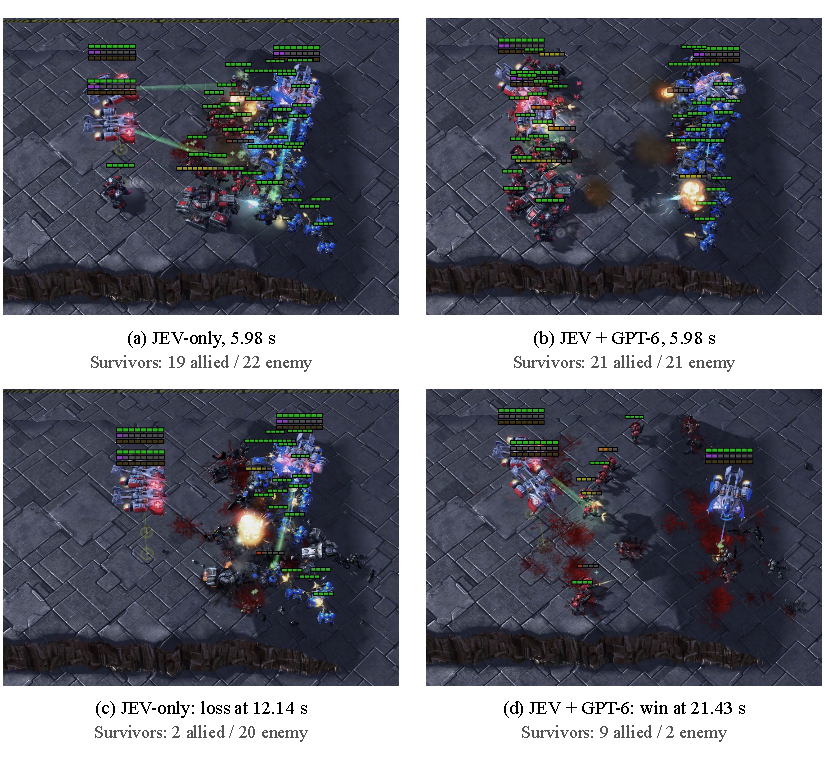
\includegraphics[width=\linewidth]{figures/micro_replay.pdf}
\caption{Replay frames from \texttt{mmmt}, episode 1. The top row shows both methods at the same game time, 5.98 seconds. The bottom row shows each episode's terminal state, at different times. Allied units are blue and opponents orange. Counts include surviving non-attacking support units, so a benchmark victory can leave enemy Medivacs alive. The same camera settings and fixed image crop are used for both columns.}
\label{fig:microreplay}
\end{figure}

\clearpage
\subsection{Full-game decision trace}

This excerpt projects recorded fields from the Lv7 seed-1 log; times and response latency are rounded. Action identifier 21 denotes building a Nexus. The observation, JEV response, command, and game result are separate events.

\lstinputlisting{listings/macro_trace.txt}

\subsection{Micromanagement plan and outcome}

These sentences are quoted from the accepted tactical plan for \texttt{mmmt}; the outcome fields come from its first episode. The plan is reused across the map's three episodes. Its requested behavior is distinct from whether each unit follows that behavior successfully.

\lstinputlisting{listings/micro_trace.txt}

\clearpage
\section{Per-map micromanagement results}
\label{app:maps}

Each map has three episodes per method. The table reports wins and mean enemy elimination; daggers identify the two local development maps. All 35 maps are included in the main 105-episode result.

\small
\begin{longtable}{lrrrr}
\caption{Complete comparison of the two methods on the same maps.}\\
\toprule
& \multicolumn{2}{c}{Wins / 3} & \multicolumn{2}{c}{Enemy elimination (\%)} \\
\cmidrule(lr){2-3}\cmidrule(lr){4-5}
Map & JEV-only & JEV + GPT-6 & JEV-only & JEV + GPT-6 \\
\midrule
\endfirsthead
\toprule
Map & JEV-only wins & Combined wins & JEV-only (\%) & Combined (\%) \\
\midrule
\endhead
\tablerows{tables/study_micro_maps.tex}
\bottomrule
\end{longtable}
\normalsize

\clearpage
\section{Cost accounting and reproducibility}
\label{app:costs}

Table~\ref{tab:individualcosts} lists the charges underlying Figure~\ref{fig:costs}. Each total is the sum of the two model components. The main combined macro average includes only the four Lv5--Lv7 games; the Lv8 stress test remains a separate completed result.

\begin{table}[h]
\caption{Individual full-game costs estimated from known token usage.}
\label{tab:individualcosts}
\centering\small
\begin{tabular}{llcrrr}
\toprule
Method & Difficulty & Seed & JEV (USD) & GPT-6 (USD) & Total (USD) \\
\midrule
\tablerows{tables/study_macro_costs.tex}
\bottomrule
\end{tabular}
\end{table}

The rates are USD~0.042 per million JEV input tokens with no output charge, and USD~10, 1, and 50 per million GPT-6 uncached input, cached input, and output tokens, respectively \citep{typesafe2026models,openai2026gpt6astra}. Cache-write input, if present, uses USD~12.50 per million. Requests exceeding 272,000 input tokens use the published long-context multipliers of two for input and 1.5 for output. We apply rates to each response before aggregation. These rates serve only to reconstruct game expenditure; the main comparison uses actual workload totals.

\begin{table}[h]
\caption{Recorded token totals for the main samples. Cached input is included in GPT-6 input. Unpriced J/G counts identify JEV/GPT-6 attempts without recorded usage; their unknown cost is omitted from the known-usage estimate.}
\label{tab:tokens}
\centering\scriptsize
\setlength{\tabcolsep}{3.5pt}
\begin{tabular}{llrrrrr}
\toprule
Setting & Method & JEV input & GPT-6 input & Cached input & GPT-6 output & Unpriced J/G \\
\midrule
\tablerows{tables/study_tokens.tex}
\bottomrule
\end{tabular}
\end{table}

The Lv8 stress test additionally contains one GPT-6 attempt without usage. A canceled planning attempt before the selected micro run also lacks usage and falls outside the completed-episode totals. Neither is treated as free. Micro planning costs are divided by three because each map's plan is reused for three episodes; they would be higher per game without reuse.

The accompanying analysis files contain 210 battle-episode records, response-level latency and usage, full-game action and state trajectories, and accepted plans. A selection manifest links these records to frozen source summaries and hashed event-log prefixes. Later appends to logs do not alter the selected data. Request latency is measured over responses with known usage; wall time comes from complete run summaries and includes setup and cleanup.

Reproduction requires the stated StarCraft II build, map files, shared-vision and ability settings, and the recorded action adapters. The initial macro catalog has 72 commands and the combined controller has 73; candidate and execution improvements are part of the system comparison. No model weights are trained.

\end{document}
